\documentclass{beamer}

\mode<presentation>
{
	\usepackage{StyleFiles/Rome}
	\setbeamercovered{transparent}
}

\mode<handout>
{
	\usepackage{pgfpages}
	\pgfpagesuselayout{2 on 1}[a4paper,border shrink=5mm]
	\nofiles
}

\usepackage[english]{babel}
\usepackage[latin1]{inputenc}
\usepackage{subfigure}
\usepackage{tikz}

\title[Alzheimer Entity Classification Combining ORB and Machine Learning]{\huge Alzheimer Entity Classification Combining ORB and Machine Learning}

\subtitle{}

\author[Fabio Previtali]{\vspace{0.1cm} \\ \large Emanuel Weitschek \\ Giovanni Felici \\ Paola Bertolazzi}

\date[May 13th 2016]{}

\begin{document}

\begin{frame}[plain]
	\begin{center}
		\LARGE
		
		\vspace{0.5cm}
		
		\textbf{Alzheimer Entity Classification Combining ORB and Machine Learning}
		
		\vspace{0.7cm}
		
		\large
		
		\emph{F. Previtali}, \emph{E. Weitschek}, \emph{G. Felici} and \emph{P. Bertolazzi}
		
		\vspace{0.2cm}
		
		\normalsize
		
		May, 13th 2016
		
		\vspace{0.5cm}
		
		\begin{center}
			\begin{tikzpicture}[map/.style={draw=black,ultra thick,inner sep=0pt}]
				\node at (0,0) [map]
				{
					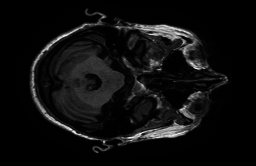
\includegraphics[height=3cm]{Figures/Brain}
				};
			\end{tikzpicture}
		\end{center}
		
		\vspace{0.5cm}
		
		\textbf{Istituto di Analisi dei Sistemi ed Informatica ``Antonio Ruberti''}
	\end{center}
\end{frame}

\section{Introduction}

\begin{frame}
	\frametitle{Challenging Problem}
	
	\begin{center}
		\begin{tikzpicture}
			\node at (0,0) [draw=white,ultra thick,inner sep=0pt]
			{
				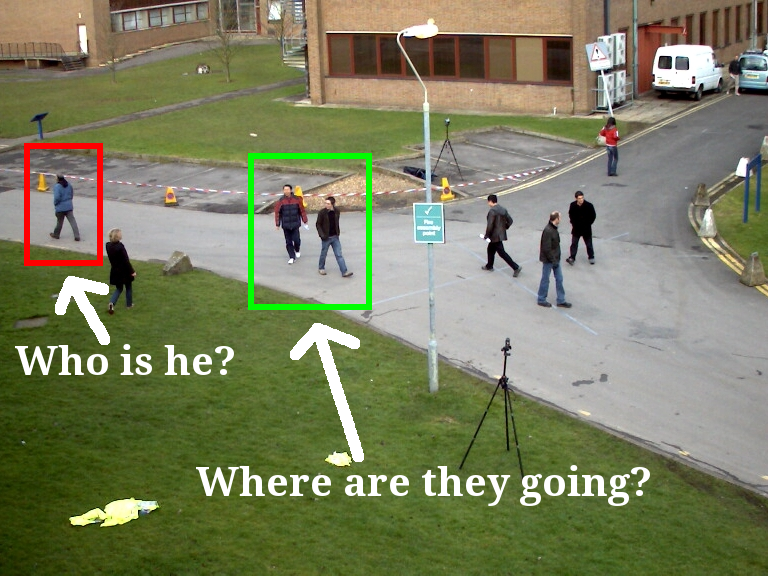
\includegraphics[width=\linewidth]{Figures/Problem.png}
			};
		\end{tikzpicture}
	\end{center}
\end{frame}

\begin{frame}
	\frametitle{Motivation}
	
	\vspace{0.2cm}
	
	\Large
	
	\begin{block}{Objective}
		\textbf{Understanding} the concept of human preference \textbf{allows} to perform higher levels
		of reasoning about future human actions. Likewise, the \textbf{knowledge} of a goal also gives
		information about \textbf{what} a person might do
	\end{block}
	
	\vspace{0.3cm}
	
	Example of application fields:
	\begin{itemize}
		\item Automatic video surveillance
		\item Human-Robot Interaction
		\item Domestic robots
	\end{itemize}
\end{frame}

\begin{frame}
	\frametitle{Contributions}
	
	\Large
	
	The main contributions of this thesis are:
	
	\begin{enumerate}
		\item \textbf{Distributed real-time} multiple object tracking
		\item \textbf{Asynchronous} and \textbf{fully} scalable design
		\item \textbf{Prediction} without prior scene semantics knowledge
		\item \textbf{Incremental} updates of the \emph{IRL} model over time
		\item \textbf{Non-uniform grids} for representing world state
		\item \textbf{Efficient} and \textbf{scalable} solution for on-robot implementation
	\end{enumerate}
\end{frame}

\begin{frame}
	\frametitle{Proposed Solution}
	
	\vspace{0.5cm}
	
	\begin{tikzpicture}
		\node at (0,0) [draw=white,ultra thick,inner sep=0pt]
		{
			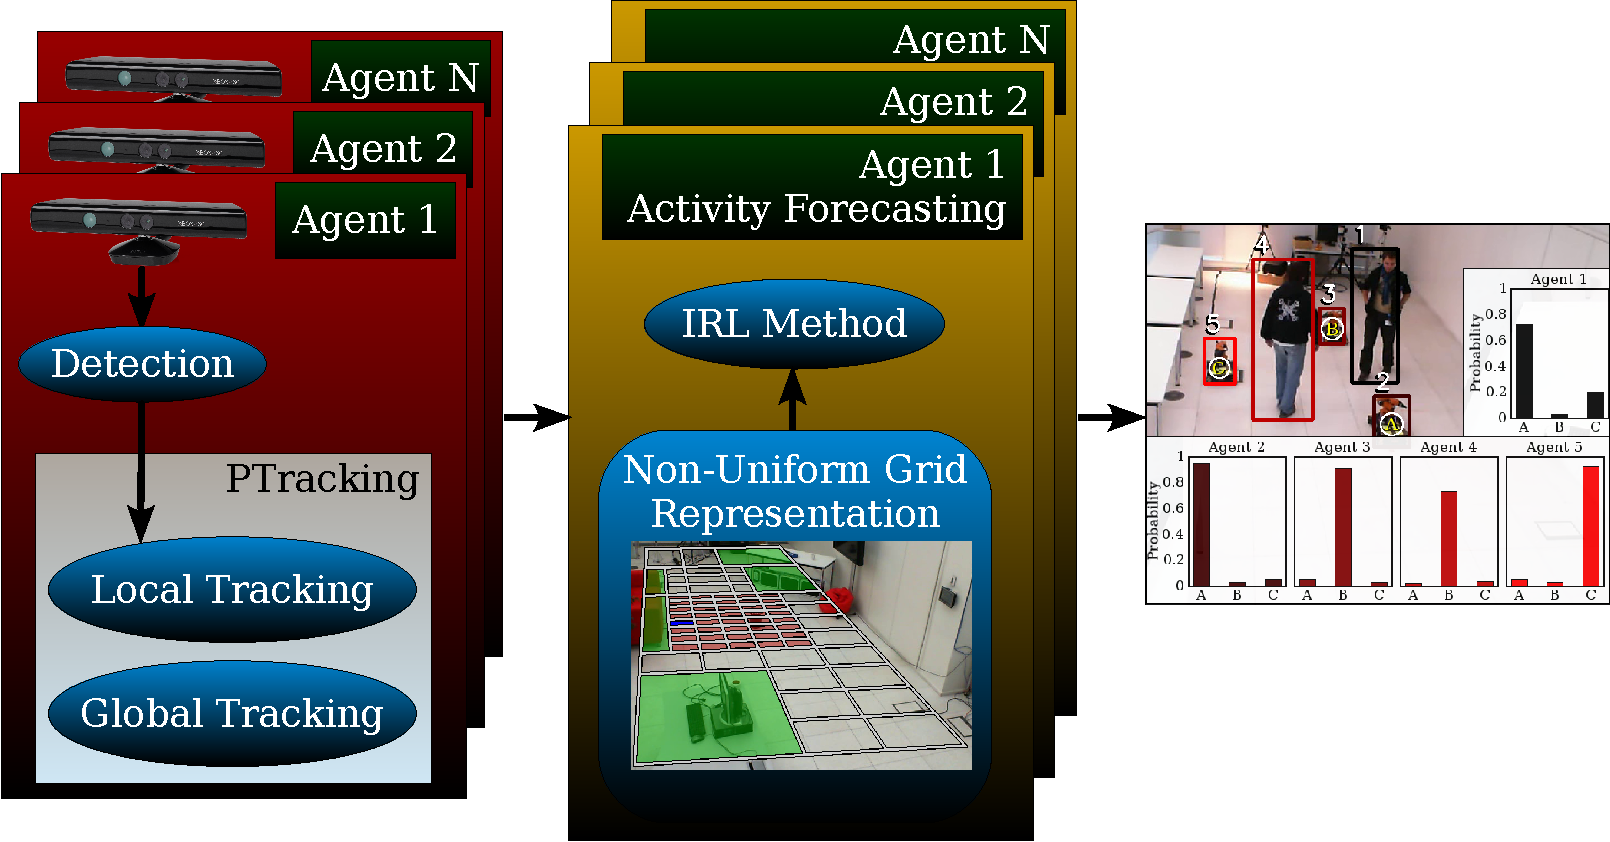
\includegraphics[width=\linewidth]{Figures/Architecture}
		};
	\end{tikzpicture}
\end{frame}

\section{Method}

\begin{frame}
	\frametitle{Contributions}
	
	\Large
	
	\vspace{0.8cm}
	
	We present an automated approach for classifying Alzheimer's disease patients from MRI brain scans.
	
	\begin{enumerate}
		\item key points extracted with a \textbf{recent} feature extraction technique, called ORB
			  \cite{Rublee11}
		\item final set of features obtained by \textbf{defining} two \textbf{new} metrics:
			  \textbf{spatial position} of extracted key points and \textbf{their distribution} around the
			  patient's brain
		\item \textbf{fast} and \textbf{reliable} approach for a straightforward deploy in clinical
			  applications
	\end{enumerate}
	
	\vspace{0.58cm}
	
	\tiny
	
	\cite{Rublee11} E. Rublee \emph{et al.}, ``ORB: an efficient alternative to SIFT or SURF'',
	International Conference on Computer Vision, 2011
\end{frame}


\end{document}
